\documentclass[12pt]{article}
\usepackage[margin=1in]{geometry}
\usepackage{fancyvrb}
\usepackage{multicol}
\usepackage{hyperref}
\usepackage{amsmath}

\usepackage[listings]{tcolorbox}

\definecolor{codegreen}{rgb}{0,0.6,0}
\definecolor{codegray}{rgb}{0.5,0.5,0.5}
\definecolor{codepurple}{rgb}{0.58,0,0.82}
\definecolor{backcolour}{rgb}{0.95,0.95,0.92}

\lstdefinestyle{mystyle}{
    language=Python,
    backgroundcolor=\color{backcolour},   
    commentstyle=\color{codegreen},
    keywordstyle=\color{magenta},
    numberstyle=\tiny\color{codegray},
    stringstyle=\color{codepurple},
    basicstyle=\ttfamily\footnotesize,
    breakatwhitespace=false,         
    breaklines=true,                 
    captionpos=b,                    
    keepspaces=true,                 
    numbers=left,                    
    numbersep=5pt,                  
    showspaces=false,                
    showstringspaces=false,
    showtabs=false,                  
    tabsize=2,
    escapechar=|,
    frame=single
}

\lstset{style=mystyle}
\begin{document}
\sloppy
\centerline{\Large CSCI 111, Lab 8}
\centerline{\large SNAKE!}

\begin{description}
\item[Due date:] Midnight, Tuesday, November 8, on Canvas.
No late work accepted.  

\item[File names:]  Names of files, functions, and variables, 
when specified,
must be EXACTLY as specified.  This includes simple mistakes such
as capitalization.

\item[Individual work:]  All work must be your own.  Do not share
code with anyone other than the instructor and teaching assistants.
This includes looking over shoulders at screens with the code open.
You may discuss ideas, algorithms, approaches, {\em etc.} with
other students but NEVER actual code.

\item[Pygame:]  First, make sure you know how pygame works.
For our purposes, it's probably best to go through the 
tutorial that results in the original (buggy) snake game:

\centerline{\url{https://www.edureka.co/blog/snake-game-with-pygame/}}

It is a very good tutorial and explains all the concepts you need
to get going. There are many other tutorials on the web that you 
can consult if you need more help:
\centerline{ \url{https://www.pygame.org/wiki/tutorials}}


\item[Hand in:]  You will write just one module for this, 
\lstinline{snake.py}, which will start with my version in the
lab folder on github.  Add your name and class information
below mine.  It is always good practice to preserve the 
lineage of a program by keeping all developers names
at the top.  

Hand in \lstinline{snake.py} on canvas by the due date.

\item[Snake:] The modified snake game is provided in the lab folder,
and includes my improvements to the original one on the web.

You will make the following improvements and additions to the game.
Add the following features in the following order.  Do not go on
to the next feature without making sure the previous one works.

\item[Game modes:]  Currently the game has three modes: playing, loser,
and quit.  These are controlled by the booleans \lstinline{loser} and
\lstinline{quitGame} (why didn't I use the name \lstinline{quit}?).

You will get rid of these booleans and have one, \lstinline{gameMode}
which can take on several values:
\begin{lstlisting}
# Game states
PLAYING = 'Playing mode'
MENU = 'Menu mode'
LOSER = 'Loser mode'
QUIT = 'Quit mode'
\end{lstlisting}
The constants (in all caps) are easier to type than the strings,
and also make sure you have fewer spelling mistakes.

Now, for example, where my code has:
\begin{lstlisting}
if quitGame:
    return()
\end{lstlisting}
you will use
\begin{lstlisting}
if gameMode == QUIT:
    return()
\end{lstlisting}
This will make it easier to control the several modes we have 
available.

Implement this step before going on.

\item[Overall game loop structure:]
For minimum pain you might want to use this structure:
\begin{lstlisting}
while not gameMode == QUIT:
    clock.tick(speed)
    for event in pygame.event.get():
        # handle user events:
        # keyboard, quit, mouse, controller, whatever
        # handling some keys may depend on gameMode
    if gameMode == QUIT:
        return()
    if gameMode == X:
        # update things X
        # display things X
    if gameMode == Y:
        # update things Y
        # display things Y
    if gameMode == Z:
        # update things Z
        # display things Z
\end{lstlisting}
    
In particular note:
\begin{itemize}
\item There is only one while loop!
\item There is only one place where we get the event queue!
\item Code updating and displaying each mode separate from other modes!
\end{itemize}

\item[Starting (and losing) menu:]
When the game begins or when the player loses a game
(there is no winning this game) there will be a menu
allowing the user to set various parameters of the game
that looks a bit like this:

\centerline{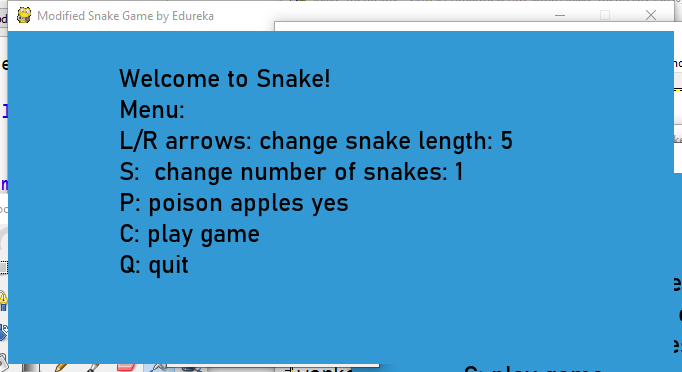
\includegraphics[scale=0.25]{menu}}

After a loss, the only thing that changes is the top line,
which changes from "Welcome" to "You lost!"

You may also want to include the score on the loser menu.

This screen will allow the user to set various configuration
parameters for the game, as follows.

\begin{description}
\item[\tt startSnakeLength]:
This has a default value of 5.  Can be set to any positive
integer with the left/right arrows.  Note that in your
keyboard handling you will have to distinguish between
\lstinline{gameMode}s to handle the arrows correctly.
\item[\tt nSnakes]:  Starting value of 1,  can be
toggled between 1 and 2 with the S key.
\item[\tt poisonApples]: Starting value of \lstinline{False},
can be toggled to \lstinline{True} with the P key.
\end{description}

Implement this feature before going on.  The toggling and changing
will change the variables, but of course nothing in the game will
change.  You can check that your menu is working by just printing
out the values of the variables each time they are changed.

\item[Poison apples:]  The game is a bit more interesting with
more kinds of food to eat.  A simple one is a food item of a different
color. If the snake eats this food, the game is over.

If the user selects this feature from the menu, add it to
the game.  This is the easiest feature to add, so do this
first.

It is straightforward to add a food item of a different color,
and end the game if the snake eats it.  To make it a bit 
more interesting the poison apple will appear and disappear
at random times.  Here is how we accomplish that.

We will introduce some new global variables:
\lstinline{poisonX} and \lstinline{poisonY}, which tell us
where to draw the poison apple, and also \lstinline{poisonOn}
initialized to \lstinline{False},
and \lstinline{poisonCount} initialized to a random integer
between \lstinline{10*speed} and \lstinline{20*speed}.

If \lstinline{poisonOn} is \lstinline{True}, then we draw
the poison apple at the position specified by \lstinline{poisonX}
and \lstinline{poisonY}.  If it is \lstinline{False} then
we don't draw it.

Every time through the game loop, the counter is decremented
by one.  When the counter gets to zero, several things happen:
\begin{itemize}
\item We choose new random values for \lstinline{poisonX},
\lstinline{poisonY} and \lstinline{poisonCount} in the 
appropriate ranges.
\item We toggle \lstinline{poisonOn} to the opposite value.
\end{itemize}
The result of these operations is that the poison apple will
appear for 10 to 20 seconds at a random location, 
then disappear for 10 to 20 seconds, then reappear at a new
location for 10 to 20 seconds, and so on.

Naturally, if the snake collides with \lstinline{poisonX}
and \lstinline{poisonY} the game is over {\bf only if}
\lstinline{poisonOn} is \lstinline{True}!

Pick a nice ugly color for the poison apple, so the user
knows which kind of food is good and which is bad.

Implement this feature before going on!

\item[Starting snake length:] 
The game is more interesting after the snake
has some length.  After the menu, create the snake
of the length specified by the user.

Create the initial snake with head
at the center of the board, and tail stretching off to
the left, like before.  You will need to create a function that
creates a snake of that length.  After the user
enters their choice in the menu, you will have to
run this function for the snake before beginning 
game play.

Note that you will have to change the starting
behavior of the snake.  What happens if you 
just start the existing game with a longer snake?  For example,
instead of:
\begin{lstlisting}
    snake = [(x1,y1)]
\end{lstlisting}
you put:
\begin{lstlisting}
    snake = [(x1-40,y1), (x1-30,y1), (x1-20,y1), (x1-10,y1), (x1,y1)]
\end{lstlisting}
what happens?  Why?

How can you fix this?  A simple way is to start the game with the snake
moving (by changing the initial
\lstinline{x1Change} value, for instance), 
throwing the player {\em en media res}.  

For this lab, you can do that, or
you can make it so the snake does not move until
the player enters the first direction.  
You will have to modify a bit of code to do this.

What happens if the user starts with a number
so big the tail goes off the board?  What can you do
about that?  I see two approaches:  prohibit such long
snakes, or allow them but don't draw any part of the snake
that is off the board.  Your choice.

Implement this feature before going on.  Make sure you handle
very long snakes!

\item[Multiple snakes:]  If the user selects two snakes,
then two snakes should appear so that two players
can play competitively.  They should have different
colors so they can be visually distinguished.

For two people to play they will have to sit side
by side and use the same keyboard.  One player will
use the arrow keys as usual, the other will use the WASD
keys.  These are standard keys used in many games so that
the left hand can control direction while the right
hand uses the mouse (no mouse needed in this game).

The mapping should be obvious from the layout:  W=UP,
A=LEFT, S=DOWN, and D=RIGHT.

The score for each player is kept and updated and displayed
at the top of the screen.  The color of the score text
should match the color of the snake so we know who's score is who's.

If either snake runs into a wall or the body of a snake
(either one), or eats a poison apple, the game is over.

This will be the hardest feature to implement, so save
this for last.

By the way, playing two snakes by yourself is a mind-bending
and frustrating challenge!  You may want to slow the game
speed down for this one.

\item[Going further:]  That's all that's required for this lab.
There are, of course, infinitely many directions you can go
with this.  Some examples:
\begin{itemize}
\item Add sounds.  A crunchy noise when the snake eats something.
A crash of broken glass when it hits the wall, followed by
a sad ``Wa-wa-waaaaa'' for the loser screen.  A dying scream
when a poison apple is eaten.

If you google ``free game sound effects'' you should find plenty.
Consult the pygame documentation to find out about loading and 
playing sounds.

\item Background music.  What game isn't identified with signature
music?  You can also find free game-style music on the web.

\item Lives.  This game only gives you one life.  Most cool
games give you a finite number of lives before ending.

\item It's a bit unfair to end the game with two snakes when
only one snake dies.  That way, if you're ahead, you can 
guarantee a win by crashing into something deliberately.

Fix this so that, when one snake dies, the other keeps going
and can run up their score.

\item More kinds of food?  Power-ups to increase your speed?
Give you invinicibility for a limited time?  Power-ups that give
you free points without adding to your tail length?  Power-downs
that deduct from your opponent's score?

\item Surely you've got some ideas of your own. 

\item Game design is fun!
Look into CSCI 319.
\end{itemize}




\end{description}
\end{document}
